\documentclass[tikz,border=10pt]{standalone}
\begin{document}
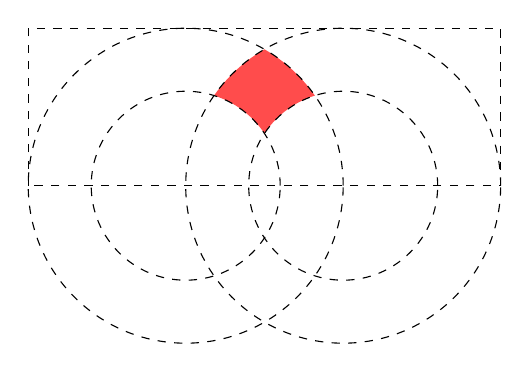
\begin{tikzpicture}[even odd rule]
  \begin{scope}
    \clip (-3,0) rectangle (3,2);
    \clip (-1,0) circle (1.2) (-1,0) circle (2);
    \fill[red!70]  (1,0) circle (1.2)  (1,0) circle (2);
  \end{scope}
  \draw[dashed] (-3,0) rectangle (3,2);
  \draw[dashed] (-1,0) circle (1.2) (-1,0) circle (2);
  \draw[dashed]  (1,0) circle (1.2)  (1,0) circle (2);
\end{tikzpicture}
\end{document}
